\documentclass[11pt]{scrartcl}
\usepackage{graphicx}
\usepackage[utf8]{inputenc}
\usepackage{amsmath}
\usepackage{listings}

\title{1. Report Multicore Systems}
\author{Simon Lermen, Ming Hong Li}

\date{\today}

\begin{document}
\maketitle
\section{Set Associative Cache}

\subsection{Calculations}

The tag, index and offset where computed in the following way:
\begin{lstlisting}
int addr   = Port_Addr.read();
int offset = (addr & 31);
int tag = (addr >> 5);
int index = (tag & 127);     
tag = (tag >> 7); 
\end{lstlisting}

\subsection{Results}

Figure~\ref{fig:waveform} shows a snapshot from the waveform file generated by the program.
The hit miss rate varied significantly between the provided tracefiles. The tracefile dbg\_p1.trf produced adresses that were much smaller than 32~bit resulting in the tag being equal to 0 most of the time.

\begin{figure}
\centering
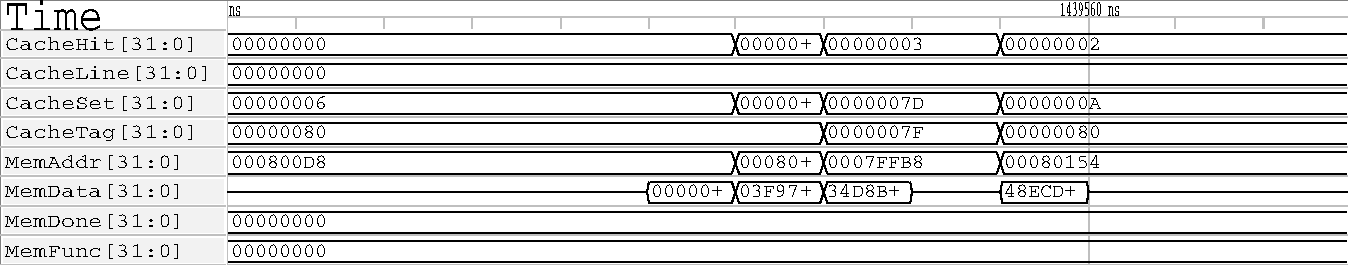
\includegraphics[scale=0.7]{./graphics/wavefilecut.pdf}
\label{fig:waveform}
\caption{Snapshot from a generated waveform file}
\end{figure}

\end{document}